\documentclass[a4paper,USenglish,anonymous]{gd-lipics-v3}
%% anonymous: for double-blind review
%% Remove "anonymous" for camera-ready version

\usepackage{graphicx}
\usepackage{svg}
\usepackage{algorithm}
\usepackage{algpseudocode}
\usepackage{booktabs}

\graphicspath{{./images/}}

\bibliographystyle{plainurl}% mandatory for LIPIcs

\title{MSAGLJS: Graph Layout, Edge Routing, and Tiling for the Web}

\author{Lev Nachmanson}{Microsoft Research, Redmond, US}{levnach@hotmail.com}{}{} 
\author{Xiaoji Chen}{}{cxiaoji@gmail.com}{}{}

\authorrunning{L. Nachmanson and X. Chen}

\Copyright{Lev Nachmanson and Xiaoji Chen}

\ccsdesc[500]{Human-centered computing~Graph drawings}
\ccsdesc[300]{Theory of computation~Computational geometry}

\keywords{Graph visualization, edge routing, Constrained Delaunay Triangulation, tiling, WebGL}

\category{Track 2, Long Paper}

\supplement{\url{https://github.com/microsoft/msagljs}}

\GAIDecl{Generative AI was used for editorial assistance in the preparation of this article.}

%% Custom macros
\newcommand{\comm}[1]{}
\newcommand{\TODO}[1]{{\color{magenta}{#1}}}
\newcommand{\cdt}{$\mathcal{T}$}
\newcommand{\unpath}{$\mathcal{L}$}
\newcommand{\triset}{$\mathcal{U}$}
\newcommand{\plg}{$\mathcal{P}$}
\newcommand{\obst}{$\mathcal{O}$}
\newcommand{\capac}{$\mathcal{C}$}
\newcommand{\mw}{$\mathcal{W}$}
\newcommand{\mh}{$\mathcal{H}$}
\newcommand{\msagljs}{\textsf{MSAGLJS}}

%% Editor-only macros (do not touch as author) %%%%%%%%%%%%%%%%%%%%%%%%%%%%%%%%%%
\EventEditors{TBD}
\EventNoEds{2}
\EventLongTitle{34th International Symposium on Graph Drawing and Network Visualization (GD 2026)}
\EventShortTitle{GD 2026}
\EventAcronym{GD}
\EventYear{2026}
\EventDate{August 19--21, 2026}
\EventLocation{Ontario, Canada}
\EventLogo{}
\SeriesVolume{42}
\ArticleNo{0}
%%%%%%%%%%%%%%%%%%%%%%%%%%%%%%%%%%%%%%%%%%%%%%%%%%%%%%

\begin{document}

\maketitle

\begin{abstract}
We present \msagljs{}, an open-source TypeScript library for graph
visualization in web browsers, distributed as a set of NPM
packages\footnote{\texttt{@msagl/core}, \texttt{@msagl/drawing},
\texttt{@msagl/parser}, \texttt{@msagl/renderer-webgl} --- all
available on \url{https://www.npmjs.com/}.}. It provides a set of
layout algorithms, a set of edge routing algorithms, and two renderers
that run in an Internet browser: one based on SVG and another based on
WebGL via the deck.gl framework. In this paper we concentrate on two
features of the latter renderer.

First, a \emph{tiling scheme} that turns a large graph into a
navigable map with \emph{semantic zoom}: at every zoom level the
labels of the highest-ranked nodes remain readable, just as the names
of major geographical features stay readable on digital maps---making
the browsing experience familiar to anyone used to online maps. Second, a
\emph{corridor routing} method that routes each edge along the
shortest path in homotopy class around the node obstacles, based on
the Constrained Delaunay Triangulation. The whole pipeline runs
client-side, without a dedicated server, on a phone or a laptop. In
this configuration the WebGL renderer interacts smoothly with graphs
of up to 10\,000 nodes and 40\,000 edges.\TODO{Re-run benchmarks to
  confirm the maximum graph size; current 10\,000 / 40\,000 figures
  are placeholders.}

\msagljs{} is available at \url{https://github.com/microsoft/msagljs}.
\end{abstract}

%% ═══════════════════════════════════════════════════════════════════
\begin{figure}[t]
  \centering
  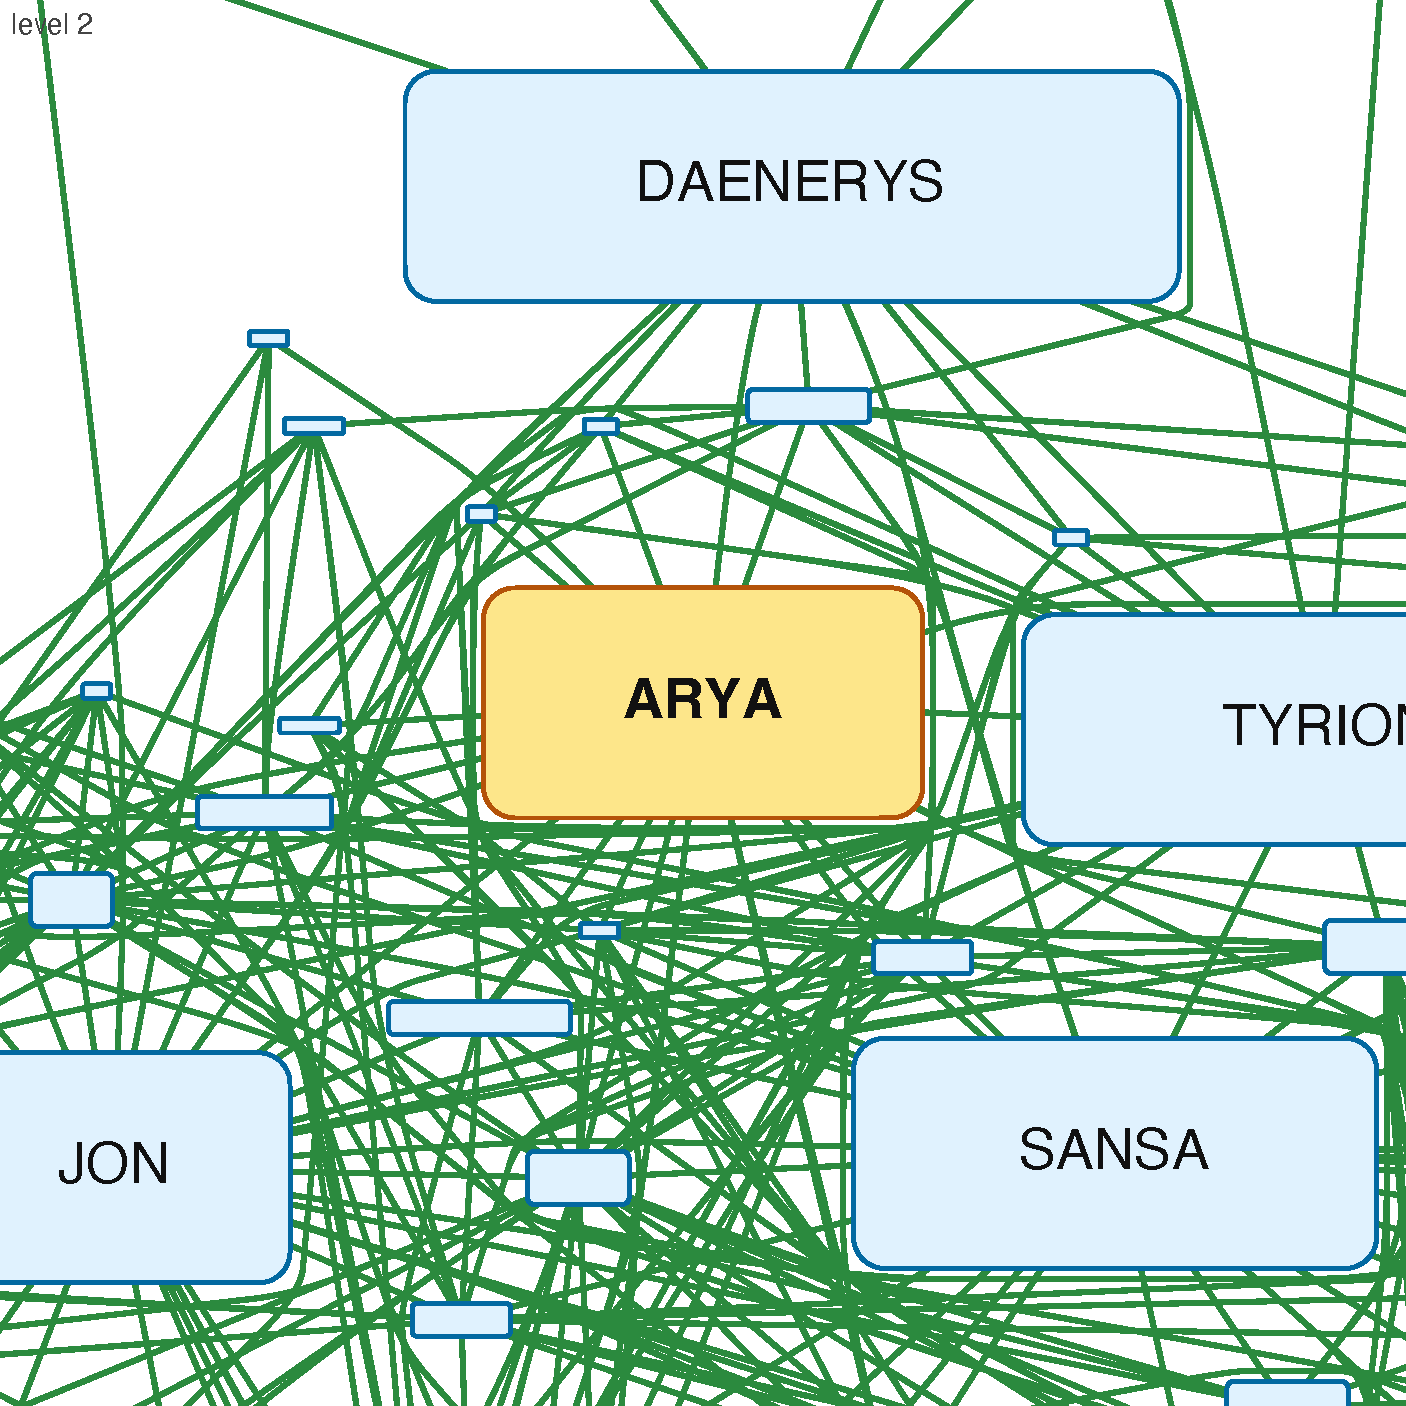
\includegraphics[width=0.48\textwidth]{tile_pyramid_coarse.pdf}\hfill
  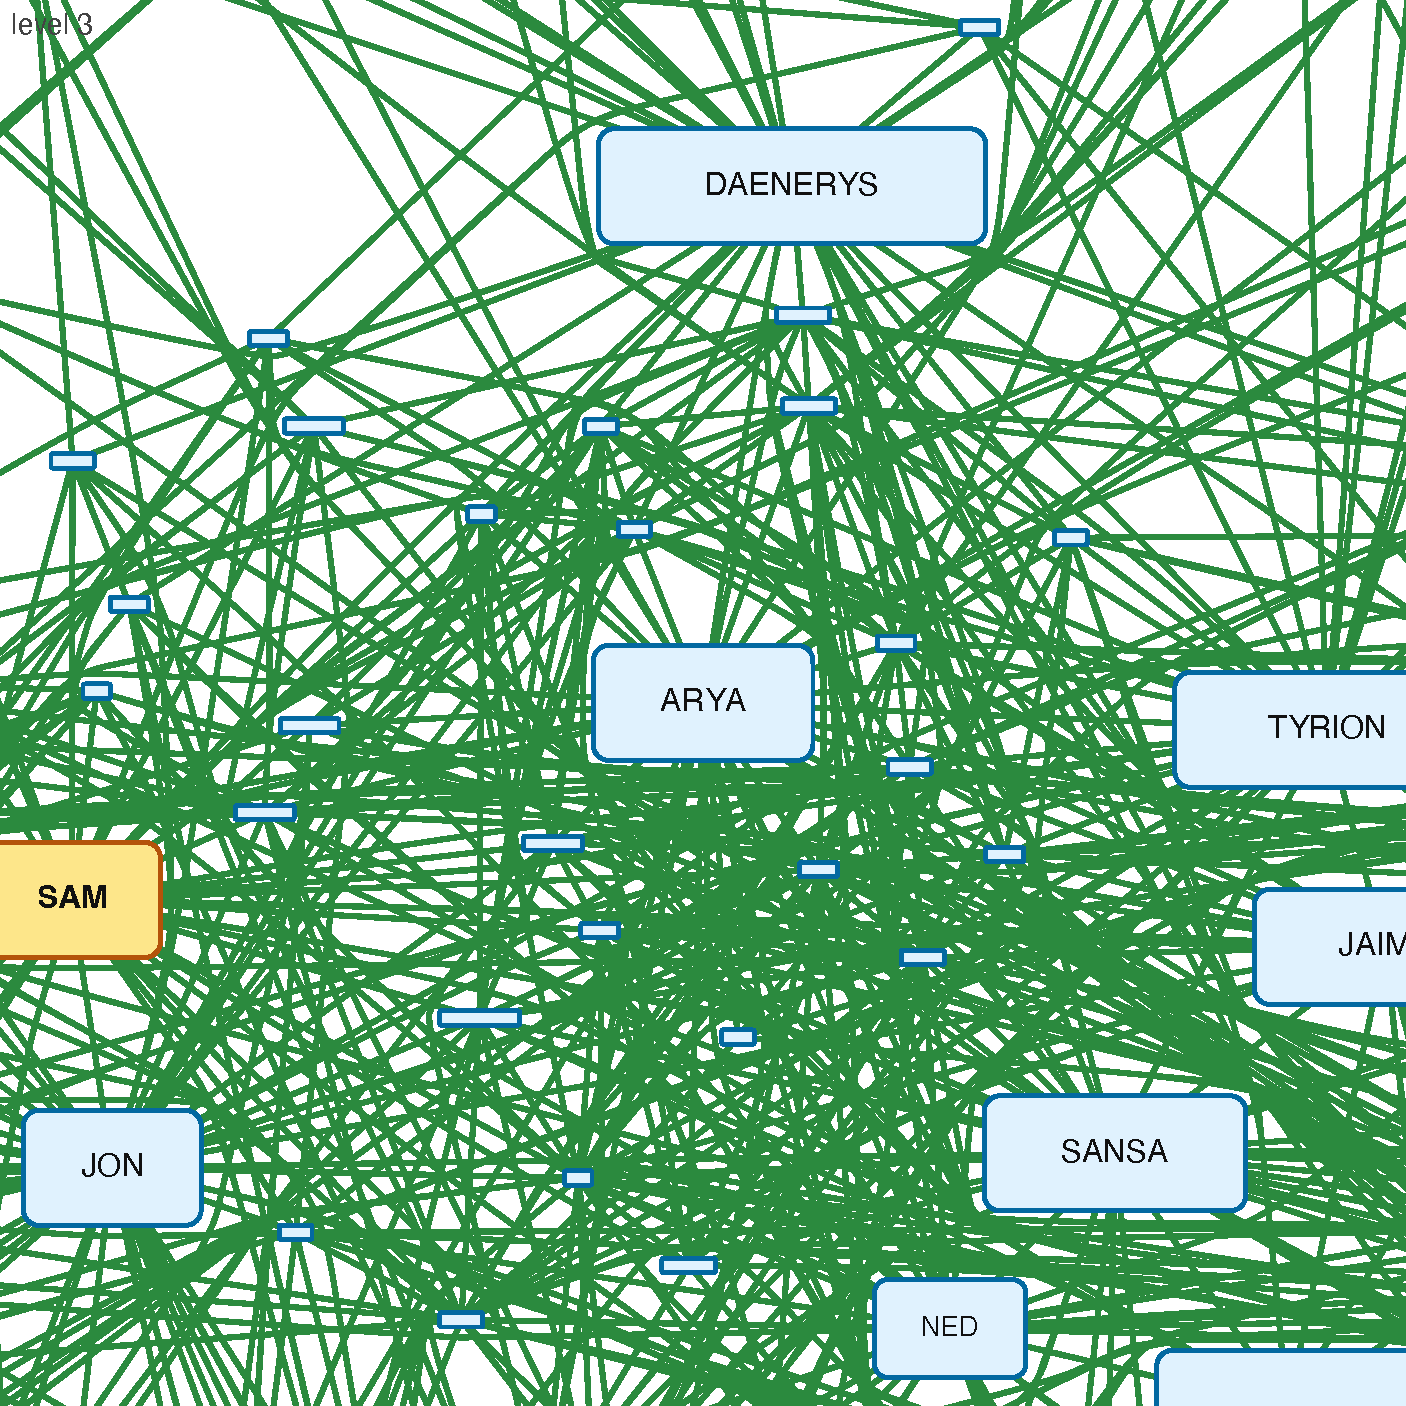
\includegraphics[width=0.48\textwidth]{tile_pyramid_fine.pdf}
  \caption{Overview of the per-level-graph tiling scheme presented in Section~\ref{sec:tiling}, on the Game of Thrones graph. Two adjacent pyramid levels are shown, cropped to the same window; the coarser level is on the left, the finer one on the right. For each level a new graph is assembled from a PageRank-ranked subset of the nodes, and the top-ranked landmark, highlighted in amber, enters that level enlarged by a factor of two in each dimension. Remaining survivors, shown in light blue, are kept at a node-specific scale~$s_v\in[0.25,\,2]$ that shrinks with rank so that they do not overlap. Edges are rerouted per level with a sleeve-hint A* built from the finer-level route, which keeps the coarse shape close to the fine one and yields smooth transitions as the user pans and zooms.}
  \label{fig:tile-pyramid}
\end{figure}

\section{Introduction}
\label{sec:intro}

Visualizing graphs in web browsers without a dedicated server presents
unique challenges: the runtime is single-threaded, the per-tab
JavaScript heap is capped at roughly 4\,GB,\footnote{In current
Chrome, V8 with pointer compression caps the per-tab JavaScript heap
at approximately $4\,\text{GB}$ ($2^{32}$ bytes).} and users expect
the smooth pan-and-zoom experience familiar from online
maps. \msagljs{}\footnote{\url{https://github.com/microsoft/msagljs}}
is an open-source TypeScript library that addresses these challenges
by combining efficient layout algorithms, a novel edge routing method,
and a tiling scheme for level-of-detail rendering.

\msagljs{} is consumed as a set of NPM packages and renders graphs using WebGL through the deck.gl framework~\cite{deckgl}. It supports the layered Sugiyama scheme~\cite{sugiyama1981}, Pivot MDS~\cite{brandes2007eigensolver}, and IPSep-CoLa~\cite{dwyer2006ipsepcola}, with edges routed around node obstacles. Throughout this paper our typical example is a social network laid out by IPSep-CoLa; the methods we describe, however, are agnostic to the layout algorithm and apply to any node placement in which the nodes do not overlap. The rendering pipeline builds a hierarchy of tiles---analogous to map tiles---so that at any zoom level only a bounded number of entities are drawn. Tiles are delivered to the browser through the standard \texttt{TileLayer} of the \texttt{@deck.gl/geo-layers} package, giving smooth pan and zoom. Live demos are available online: a WebGL renderer for large graphs\footnote{\url{https://microsoft.github.io/msagljs/renderer-webgl/index.html}} and an SVG renderer for smaller, editable graphs\footnote{\url{https://microsoft.github.io/msagljs/renderer-svg/index.html}}.

This paper makes two main contributions:
\begin{enumerate}
\item A \emph{tiling scheme} for large graph visualization that builds a hierarchical tile pyramid, limits visible entities per tile using PageRank-based filtering, simplifies edge routes at coarser levels, and integrates with the WebGL renderer for real-time pan and zoom.
\item A \emph{corridor routing} algorithm that routes edges on the dual graph of a Constrained Delaunay Triangulation, using per-source batched Dijkstra trees followed by the classical funnel algorithm to produce shortest-path geodesics in homotopy classes.
\end{enumerate}

%% ═══════════════════════════════════════════════════════════════════
\section{Related Work}
\label{sec:related}

\paragraph{Graph visualization tools.}
Graphviz~\cite{gansner2000graphviz,graphviz} is a long-standing graph
drawing tool supporting multiple layout algorithms, including the
Sugiyama method and Scalable Force-Directed Placement~\cite{sfdp}; it
does not support tiling or WebGL rendering. Our library builds on the
earlier MSAGL desktop layout engine~\cite{nachmanson2004glee} that did
not have the features described here. On the web,
Sigma.js~\cite{sigmajs} and Cytoscape.js~\cite{franz2016cytoscape}
provide interactive graph rendering, but rely on straight-line or
generic spline edges without obstacle-avoiding routing and without a
pyramid of precomputed tiles. ReGraph~\cite{regraph} uses WebGL to
render large graphs with straight-line edges and supports interactive
cluster expansion but not tiling. Cosmograph~\cite{cosmograph} uses
GPU-accelerated force-directed layout for million-node graphs with
straight-line edges, without
tiling. GraphMaps~\cite{nachmanson2015graphmaps} supports tiling and
level-of-detail for large graphs but runs only on Windows and does not
optimize edge routes. Cornac~\cite{perrot2018cornac} handles huge
graphs with tiles and edge
bundling~\cite{hurter2012graph,holten2009fdeb} but requires a
multi-server backend. Earlier navigation schemes for large graphs
include ASK-GraphView~\cite{abello2006askgraphview}, which organizes
nodes into a hierarchical cluster tree, and topological fisheye
views~\cite{gansner2005topological}, which distort a multilevel
layout~\cite{harel2002multiscale,hu2005efficient} under the focus;
neither targets browser-side tile pyramids or per-level edge
rerouting. Hierarchical edge bundling~\cite{holten2006hierarchical}
and force-directed bundling~\cite{holten2009fdeb} are complementary
clutter-reduction techniques applied \emph{after} edges have been
routed.

\paragraph{Shortest paths and edge routing.}
Our corridor algorithm walks the dual of a Constrained Delaunay
Triangulation~\cite{shewchuk2002delaunay} and relies on the classical
funnel algorithm for extracting a geodesic from a triangle
strip~\cite{lee1984euclidean,chazelle1982theorem,guibas1987linear,pathOpt}.
The optimal algorithm for Euclidean shortest paths among polygonal
obstacles~\cite{hershberger1999optimal} and the recent
$O(m\log^{2/3} n)$ single-source shortest-path algorithm that breaks
the sorting barrier~\cite{duan2025sorting} are remarkable theoretical
results, but they are not practical: both build elaborate global data
structures that we avoid.
Graphviz builds the full visibility graph for edge routing in force-directed layouts, which has $O(n^2)$ edges. For Sugiyama layouts, it uses the funnel algorithm~\cite{dobkin1997implementing} but requires a simple containing polygon. yWorks~\cite{yworks} offers ``Organic edge routing'' based on force-directed simulation. The approach of Dwyer and Nachmanson~\cite{dwyer2010fast} routes on a Yao-graph spanner with local shortcutting. For orthogonal layouts, the libavoid framework of Wybrow, Marriott and Stuckey performs obstacle-avoiding connector routing with incremental updates~\cite{wybrow2010orthogonal}. Our corridor method eliminates the spanner entirely and routes directly on the CDT dual graph, and is, to our knowledge, the first routing algorithm integrated with a browser-side tile pyramid that reroutes edges per level.


%% ═══════════════════════════════════════════════════════════════════
\section{System Architecture}
\label{sec:arch}

\msagljs{} is organized as a monorepo with five NPM packages:

\begin{description}
\item[\texttt{@msagl/core}] --- Graph data structures, layout algorithms (Sugiyama, MDS, IPSep-CoLa), edge routing, CDT, tiling.
\item[\texttt{@msagl/drawing}] --- Visual attributes (colors, shapes, labels) bridging the graph model and renderers.
\item[\texttt{@msagl/parser}] --- Parsers for DOT and JSON graph formats.
\item[\texttt{@msagl/renderer-svg}] --- SVG-based renderer for small graphs.
\item[\texttt{@msagl/renderer-webgl}] --- WebGL renderer using deck.gl~\cite{deckgl}, with tiling support.
\end{description}

The layout pipeline proceeds in three phases:
\begin{enumerate}
\item \textbf{Layout.} Node positions are computed by the chosen algorithm. For large undirected graphs the default is force-directed layout (IPsepCola) initialized with Pivot MDS~\cite{brandes2007eigensolver}; for directed graphs, Sugiyama layout is used.
\item \textbf{Edge routing.} Edges are routed around node obstacles. The routing mode is configurable; this paper focuses on \emph{corridor routing} (Section~\ref{sec:corridor}).
\item \textbf{Tiling.} A tile hierarchy is built for level-of-detail rendering (Section~\ref{sec:tiling}).
\end{enumerate}

The WebGL renderer (Section~\ref{sec:webgl}) consumes the tile hierarchy and renders the appropriate level of detail based on the current viewport.

%% ═══════════════════════════════════════════════════════════════════
\section{Tiling}
\label{sec:tiling}

To visualize large graphs interactively, \msagljs{} builds a pyramid
of tiles analogous to those used in online maps, served to the browser
through the \texttt{TileLayer} of the \texttt{@deck.gl/geo-layers}
package~\cite{deckglTileLayer}. Levels are numbered $0,1,\dots,Z$ from
coarsest to finest; level~$0$ is a single tile covering the whole
drawing with only a few top-ranking graph features,
and the finest level~$Z$ corresponds to the full graph
produced by the layout and the corridor router of
Section~\ref{sec:corridor}.

Conceptually, each tile is associated with a rectangular viewport and
holds the graph elements that lie within it: the single tile at
level~$0$ is associated with a viewport covering the entire drawing,
so it contains the whole graph. When rendering, every level shows only
a prefix of the graph elements ranked by importance, and each tile
renders the part of that prefix that lies within its viewport; the
remaining elements are hidden. The per-tile capacity~$\mathcal{C}$
only governs the choice of $Z$ (when to stop subdividing) and is not
consulted when deciding what to render at each level: the selection of
visible elements per level is driven entirely by importance and
geometric non-overlap (Section~\ref{sec:filter}). Only the finest
level~$Z$ displays every node and edge of the graph.

\emph{Per-tile rendering load.} At the finest level, condition~(i) is
intended to cap each tile at $\mathcal{C}$ visible elements (nodes
plus edge clips, default $\mathcal{C}=500$). On dense graphs, however,
either the depth cap $Z_{\max}=8$ or the minimum tile size~(ii) binds
first, in which case the densest finest-level tile may hold many more
than $\mathcal{C}$ elements. For a coarser level~$z<Z$ we ignore
$\mathcal{C}$ when preparing a tile for rendering. We apply semantic
zoom on the nodes, (Section~\ref{sec:filter}) by inflating each
surviving node by roughly $2^{Z-z}$ in linear size. The chosen nodes
define the rendered edges: we render the edges connecting two chosen
nodes. Table~\ref{tab:max-per-tile} reports the
empirical worst-case per-tile element count on a range of graphs.

\paragraph{How $Z$ is chosen.} $Z$ is determined incrementally rather
than fixed in advance. We initialize $Z=0$ with the single root tile
covering the whole drawing. While the tiles at level~$Z$ violate
conditions~(i)~or~(ii) below, we increase $Z$ by one and split every
tile of the previous finest level into four equal sub-tiles. The two
conditions are: (i)~every tile contains at most~$\mathcal{C}$ visible
elements (default $\mathcal{C}=500$), preventing overloaded tiles; and
(ii)~the tile width and height are both below ten times the average
node width and height, preventing tiles smaller than the nodes they
display. We additionally enforce a hard cap $Z \le Z_{\max}$ derived from a
memory estimate. At level~$z$ the pyramid has a $2^{z}\times 2^{z}$
grid of tiles, so the finest grid resolution is $K = 2^{Z}$. Across
the whole pyramid we estimate the total number of stored tile elements
as
\[
T(K) \;\approx\; 2\,\bigl((K/4)\,M + N\bigr),
\]
where $N$ and $M$ are the node and edge counts of $G$. The term
$(K/4)\,M$ counts per-tile edge clips at the finest level, under the
heuristic that an average edge crosses $K/4$ tiles. The additive $N$
counts node copies. The factor~$2$ accounts for the contribution of
all coarser levels combined. With roughly $200$~bytes per stored
element and a maximum memory $\mathcal{M}_{\max}$ (default $4$~GB), we
solve $200\,T(K) \le \mathcal{M}_{\max}$ for the largest admissible
$K$,
\[
K_{\max} \;=\; \Bigl\lfloor\,4\bigl(\mathcal{M}_{\max}/(2\cdot 200) - N\bigr)\big/M\,\Bigr\rfloor,
\]
and set
\[
Z_{\max} \;=\; \min\!\bigl(8,\;\bigl\lfloor\log_2 K_{\max}\bigr\rfloor\bigr).
\]
The constant $8$ is a safety ceiling: even when $\mathcal{M}_{\max}$
allows a much larger grid, we never build more than nine pyramid
levels.
\paragraph{Three phases.} Once $Z$ and the tile rectangles are fixed,
construction proceeds in three phases for every coarser level
$z=Z{-}1, Z{-}2, \dots, 0$: (1)~use PageRank to pick the nodes shown
at level~$z$ and possibly enlarge them
(Section~\ref{sec:filter}); (2)~reroute the edges of $G_z$ around
these obstacles, which may now be enlarged,
(Section~\ref{sec:level-reroute}); (3)~recompute the per-tile edge
clips at level~$z$ by splitting the new curves at tile boundaries
(Section~\ref{sec:tile-build}). Figure~\ref{fig:tile-pyramid} on the
first page shows two adjacent pyramid levels built by this procedure.
Algorithm~\ref{alg:build-pyramid} summarizes the whole pipeline.

\begin{algorithm}[t]
\caption{\textsc{BuildTilePyramid}$(G, \mathcal{C}, \mathit{minTileSize})$}
\label{alg:build-pyramid}
\begin{algorithmic}[1]
\State $T_0 \gets$ single tile holding all of $G$ clipped to its bounding box
\State $\mathit{levels} \gets [\,T_0\,]$;\quad $z \gets 0$
\While{some tile in $\mathit{levels}[z]$ exceeds $\mathcal{C}$ elements \textbf{and} its width/height $\ge \mathit{minTileSize}$}
  \State $\mathit{levels}[z{+}1] \gets$ split every tile of $\mathit{levels}[z]$ into four sub-tiles
  \State within each parent, distribute nodes/labels/arrowheads by bbox, and split each edge clip at the tile midlines (Section~\ref{sec:tile-build})
  \State $z \gets z + 1$
\EndWhile
\State $Z \gets z$;\quad $V_Z \gets V(G)$;\quad $s_v^{(Z)} \gets 1$ for all $v\in V_Z$
\State compute $\mathrm{PageRank}(G)$
\For{$z = Z-1$ \textbf{down to} $0$}
  \State $(V_z, \{s_v^{(z)}\}) \gets$ \textsc{SelectTopKWithAdaptiveScale}$(V_{z+1},\, 2^{Z-z})$ \Comment{Section~\ref{sec:filter}}
  \State build a CDT from the inflated polylines of $V_z$ at scales $\{s_v^{(z)}\}$
  \State reroute every edge $e\in E_z$ on this CDT, using the level-$(z{+}1)$ route as a sleeve hint \Comment{Section~\ref{sec:level-reroute}}
  \State for every tile $t$ at level $z$, recompute the clips of $e$ inside $t$ from the new curve, splitting at tile midlines
\EndFor
\State \Return $\mathit{levels}$
\end{algorithmic}
\end{algorithm}

\subsection{PageRank-Guided Level Construction}
\label{sec:filter}

To keep labels readable at coarse zooms, each level~$0 \le z < Z$ is
assigned its own \emph{level graph}~$G_z=(V_z,E_z)$: a subset
$V_z\subseteq V_{z+1}$ of active nodes together with every edge of~$G$
whose endpoints both lie in~$V_z$. We compute
PageRank~\cite{page1999pagerank} on~$G$ once, sort all nodes by
descending PageRank as $v_0,v_1,\dots,v_{|V|-1}$ and write $S_z = 2^{\,Z-z}$ for
the per-level scale ceiling.

\paragraph{Building $V_z$.}
The intuition is a greedy seniority sweep: highly ranked nodes ``claim'' as much screen room as the level allows, and lower-ranked ones squeeze into whatever space is left. Concretely, the candidate set at level~$z$ is the rank-prefix
\[
T_z \;=\; \{\,v_0,v_1,\dots,v_{n_z-1}\,\},\qquad n_z=\bigl\lceil |V|/2^{\,Z-z}\bigr\rceil,
\]
i.e.\ a fixed-size prefix of the \emph{globally} rank-sorted node list, halving in size with each coarser level. We process $T_z$ in rank-descending order. Each candidate~$v$ is assigned the largest scale~$s_v\le S_z$ at which its bounding box, scaled about $v$'s center and inflated by a margin~$m$ that absorbs the obstacle padding used by the corridor router (Section~\ref{sec:corridor}) and leaves a visible gap between obstacles after triangulation, stays disjoint from the inflated boxes of every already-accepted node. Disjointness is a closed-form, axis-aligned separating-axis test, so $s^\star(v)$ is obtained directly from box centers and dimensions; if $s^\star(v)\ge 1$ the candidate is accepted at $s_v=\min(\sigma, s^\star(v))$, where the running cap~$\sigma$ (initially $S_z$) is then tightened to~$s_v$ to forbid any later, lower-ranked node from being drawn larger than its accepted seniors. Because $v_0$ is processed first against an empty accepted set, it always survives at the full scale~$S_z$. The accepted set becomes~$V_z$ and the per-node scales~$\{s_v^{(z)}\}$ are stored for the level. Because $T_z\subseteq T_{z+1}$ and at coarser levels boxes are only larger (so an already-tight overlap configuration cannot become looser), acceptance is monotone in~$z$: $V_z\subseteq V_{z+1}$, as required by the level-graph definition. The result is the intended map-like effect: a few large landmarks at coarse zooms, progressively more detail as the user zooms in, and a guaranteed visible gap of at least~$2m$ between every pair of un-inflated scaled boxes.

To avoid testing every candidate against every previously accepted box, accepted boxes are maintained in a uniform spatial hash whose cell size is an upper bound on the inflated box dimension at the current level. Two boxes can overlap only if their center cells are within one step on each axis, so each candidate consults at most nine cells. On the layouts we tested the expected work per candidate is~$O(1)$, giving an overall expected cost of $O(|T_z|\log|T_z|)$ dominated by the initial sort; the worst case, when many boxes pile into a single cell, degrades to $O(|T_z|\cdot|V_z|)$.

\subsection{Stable Per-Level Rerouting with a Routing Hint}
\label{sec:level-reroute}

Because $G_{z-1}$ has fewer obstacles than $G_z$, and different ones on account of the enlargement of~$v_0$, edges of~$G_{z-1}$ must be rerouted: the finest-level curves would otherwise pierce the enlarged landmark boxes. We rerun the corridor router (Section~\ref{sec:corridor}) on the active edges of $G_{z-1}$, but with two modifications that secure visual stability during zoom.

\paragraph{Per-level CDT.} For level~$z-1$ we build a dedicated CDT from the inflated polylines of~$V_{z-1}$ only, using each node's level-$z{-}1$ scale. The global landmark~$v_0$ thus enters the triangulation as an obstacle that is $2^{Z-z+1}\!\times$ its finest-level size in each dimension, so routes naturally bend around it.

\paragraph{Routing hint.} For every edge~$e\in E_{z-1}$ we already have a route~$c_e$ computed at the finer level~$z$. We sample~$c_e$, locate the CDT triangles it visits at level~$z-1$, and expand this sequence by one neighbor hop to obtain a triangle \emph{sleeve}~$S_e$. Instead of the per-source Dijkstra trees of Section~\ref{sec:dijkstra}, which are efficient when many edges share a source but ignore the previous level's shape, we run a per-edge \textbf{A*} on the dual of the level-$z{-}1$ CDT, \emph{restricted to}~$S_e$, with the source and target obstacle triangles always admissible. The hint keeps the coarse-level route topologically and geometrically close to the fine-level one, so that as the user zooms out an edge deforms smoothly rather than jumping to a different side of a landmark. If the masked A* fails, for instance when the target now lies inside the inflated landmark, we fall back to unconstrained A* on the whole dual, and finally to A* with the obstacle-interior guard disabled; all three tiers share the same pre-allocated open-set arrays.

To summarize the division of labor: \textbf{Dijkstra trees}, Section~\ref{sec:dijkstra}, drive the \emph{finest-level} routing, where there is no hint and many edges share sources; \textbf{A*} drives the \emph{per-level rerouting} for $z<Z$, where each edge carries its own sleeve hint from the finer level and independent searches are required.

\subsection{Splitting Edges between Tiles}
\label{sec:tile-build}

Once each level $G_z$ has its final geometry, we cut that level into tiles. A tile is a pair $(\mathit{rect}, \mathit{tiledata})$, where $\mathit{tiledata}$ is a set of \emph{tile elements}: nodes, edge labels, edge arrowheads, and \emph{edge clips}. An edge clip is a pair $(e, p)$, with $p$ a continuous piece of the edge curve $c_e$ confined to $\mathit{rect}$.

The single tile at level~$0$ is obtained by clipping every element to the graph's bounding box. To build level~$z+1$ from level~$z$, each tile is split into four equal sub-tiles; nodes, labels, and arrowheads are assigned to sub-tiles by bounding-box intersection, and each edge clip is cut at the tile midlines, producing sub-clips confined to individual sub-tiles. We maintain invariant~$\mathcal{F}$: (a)~every clip stays inside its tile's rectangle, crossing the boundary only at its endpoints; (b)~the union of all clips for edge~$e$ inside a tile equals $c_e \cap \mathit{rect}$.
Invariant~$\mathcal{F}$ serves two purposes. Part~(a) makes subdivision cheap and local. Suppose a parent tile has rectangle $\mathit{rect}$ with horizontal and vertical midlines $\ell_h, \ell_v$. To split a clip $(e,p)$ into its children, we collect all intersections of the underlying curve $c_e$ with $\ell_h$ and $\ell_v$, restrict them to the parameter range $[\mathit{start},\mathit{end}]$ defining $p$, sort these parameters, and prepend $\mathit{start}$ and append $\mathit{end}$. This yields a sorted parameter list $\mathit{start}=t_0<t_1<\dots<t_m=\mathit{end}$, and the $m$ child sub-clips are exactly the curve pieces over consecutive intervals $[t_{u},t_{u+1}]$. Each piece is assigned to one of the four children by sampling $c_e$ at the midpoint $(t_u+t_{u+1})/2$ and comparing against the midlines. Crucially, no intersection with the four outer sides of $\mathit{rect}$ is ever computed: invariant~(a) guarantees that the curve already lies inside $\mathit{rect}$ between $t_0$ and $t_m$ and crosses its boundary only at those endpoints, so the midlines alone fully decompose the clip into rectangle-confined pieces. This reduces subdivision to one curve--line intersection per midline plus a sort, instead of a full 2D rectangle clip.
Part~(b) is the rendering-correctness condition: at any zoom only the tiles intersecting the viewport are fetched and their clips drawn, and (b) guarantees that the union of what is drawn equals $c_e\cap\text{viewport}$ for every visible edge~$e$, so no segment is missed and none is drawn twice. The same invariant is also what makes the rerouting of Section~\ref{sec:level-reroute} compatible with tiling: whenever an edge curve~$c_e$ is replaced by a coarser-level route, (b) is reestablished by recomputing the clips of that edge inside every affected tile before the level is served.

Subdivision of a level stops as soon as either of the following holds: (i)~every tile at that level already contains at most \capac{} elements; or (ii)~the tile width and height have both dropped below ten times the average node width and height, respectively. These are the same conditions that determine $Z$ (Algorithm~\ref{alg:build-pyramid}).

Table~\ref{tab:max-per-tile} reports the resulting maximum number of elements rendered in a single tile across the entire pyramid for a range of graphs.

% Auto-generated by maxPerTile.spec.ts
\begin{table}[t]
\caption{Maximum number of elements rendered in a single tile across the pyramid (capacity $\mathcal{C}=500$; no explicit cap on $Z$, depth determined by the natural stops of Section~\ref{sec:tiling}).}
\label{tab:max-per-tile}
\centering
\begin{tabular}{lrrrrr}
\toprule
Graph & $|V|$ & $|E|$ & Levels & Max per tile & Max level \\
\midrule
gameofthrones & 407 & 2639 & 5 & 324 & 4 \\
composers & 3405 & 13832 & 8 & 696 & 3 \\
facebook\_combined & 4039 & 88234 & 9 & 961 & 5 \\
ca-GrQc & 5242 & 28968 & 8 & 304 & 4 \\
ca-HepTh & 9877 & 51946 & 8 & 1839 & 3 \\
ca-CondMat & 23133 & 186878 & 8 & 2920 & 3 \\
ca-HepPh & 12008 & 236978 & 9 & 2916 & 3 \\
deezer\_europe & 28281 & 92752 & 8 & 2395 & 3 \\
delaunay\_n15 & 32768 & 98274 & 8 & 283 & 7 \\
\bottomrule
\end{tabular}
\end{table}


%% ═══════════════════════════════════════════════════════════════════
\section{Corridor Routing on the CDT}
\label{sec:corridor}

We describe an edge routing method that routes edges directly on the dual graph of a Constrained Delaunay Triangulation, without requiring a spanner graph. The method finds a \emph{corridor}---a sequence of adjacent CDT triangles from source to target---and applies the funnel algorithm to produce the shortest path within it.

\subsection{CDT Construction and the Dual Graph}

Given the graph layout, each node is covered by a padded obstacle polygon. We compute a Constrained Delaunay Triangulation \cdt{} on the set \obst{} of these obstacle polygons~\cite{delaunay1934sphere,domiter2008sweep}. The \emph{dual graph} $D$ of \cdt{} has one node per triangle and one edge for each pair of triangles sharing a side. A triangle is \emph{free-space} if it is not contained in any obstacle interior. Each triangle of an A* (or Dijkstra) path is entered through one shared edge and left through another; the cost of the step taken inside the triangle is the Euclidean distance between the midpoints of those two edges. For the source triangle, which has no entering edge, the centroid is used as the entry point.

\subsection{A* Search on the Dual Graph}
\label{sec:astar}

Intuitively, the CDT partitions free space into triangular ``rooms'' connected by shared edges acting as ``doorways''. Routing an edge from~$s$ to~$t$ then splits into two subproblems: a \emph{combinatorial} one---which sequence of rooms to traverse---and a \emph{geometric} one---which exact polyline through that sequence is shortest. We solve the first with a best-first search on the dual graph, and the second with the classical funnel algorithm. The dual-graph search ignores fine geometry and only commits to a corridor; the funnel then pulls the path taut inside that fixed corridor, sliding it against diagonal endpoints until it is locally straight. Because A* on the dual uses centroid-to-centroid step costs and a straight-line heuristic to the target, it is consistent and returns a corridor whose total cost lower-bounds, but closely tracks, the true shortest path---good enough to feed the funnel without chasing exact geometry inside the search.
 
Concretely, for each graph edge from source~$s$ to target~$t$, we locate the containing triangles and run A*~\cite{hart1968formal} on the dual graph~$D$. The heuristic is the straight-line distance from the current centroid to~$t$. Triangles inside obstacles (other than the source and target obstacles) are excluded from the search. The resulting corridor is passed to the funnel algorithm~\cite{chazelle1982theorem,hershberger1994computing}, which computes the shortest path through the corridor's sequence of diagonals.

\subsection{Vertex Collapse at Source and Target}
\label{sec:collapse}

The corridor passes through triangles whose vertices lie on the padded obstacle boundaries. When these vertices appear as diagonal endpoints, the funnel algorithm produces sharp zigzag turns near each endpoint. We eliminate these artifacts by \emph{collapsing} obstacle vertices: any diagonal endpoint belonging to the source obstacle is replaced with the source center~$s$, and similarly for the target. Degenerate diagonals (both endpoints collapsed to the same point) are removed. The left/right orientation of each diagonal is preserved from the uncollapsed geometry.

After collapse, the funnel sees a wide opening at each endpoint and naturally selects the optimal exit direction. A final arrowhead-trimming step clips the path at the node boundary curves.

\begin{figure}[t]
  \centering
  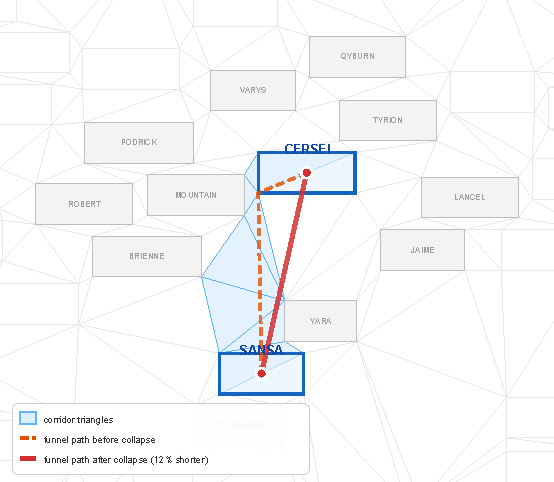
\includegraphics[width=0.65\textwidth]{collapse_CERSEI_SANSA.pdf}
  \caption{Effect of vertex collapse on the CERSEI--SANSA edge. Light blue: corridor triangles. Orange dashed: funnel path before collapse (3 waypoints). Red solid: funnel path after collapse (2 waypoints, 12\% shorter). Collapsing obstacle vertices to the node center widens the funnel opening and removes the detour.}
  \label{fig:collapse}
\end{figure}

\subsection{Batched Routing with Dijkstra Trees}
\label{sec:dijkstra}

When a node has many incident edges, running independent A* searches is wasteful. We group edges by source node and run a single Dijkstra computation per source on the dual graph, expanding until all target triangles are reached. Corridors are recovered by following parent pointers. This reduces the number of searches from $m$ (edges) to at most $n$ (nodes). On the Game of Thrones social network (407 nodes, 2\,639 edges, 331 distinct sources), the Dijkstra tree approach reduces routing time by 30\%.

%% ═══════════════════════════════════════════════════════════════════
\section{The Portal Graph}
\label{sec:portals}

The batched Dijkstra approach of Section~\ref{sec:dijkstra} still requires exploring much of the CDT for each source node. To enable faster queries, we introduce the \emph{portal graph}---an abstraction that separates the free-space routing problem from the local obstacle traversal.

\subsection{Portal Triangles}

For each node obstacle, we identify its \emph{portal triangles}: the free-space CDT triangles that share an edge with the obstacle boundary. Formally, a triangle~$t$ is a portal of obstacle~$O$ if $t$ is free-space and at least two of its three CDT sites belong to~$O$'s boundary polyline. Portals serve as entry and exit points: any shortest path from the interior of~$O$ to free space must pass through a portal triangle.

\subsection{Structure of the Portal Graph}
\label{sec:portal-structure}

The portal graph $G_P$ is defined as follows:
\begin{itemize}
\item \textbf{Nodes.} For each graph node~$v$, the center point~$c_v$ and all portal triangles $\{p_1^v, p_2^v, \ldots\}$ of $v$'s obstacle are nodes of~$G_P$.
\item \textbf{Interior edges.} Each center~$c_v$ is connected to every portal~$p_i^v$ of the same obstacle, with weight equal to the BFS distance through the obstacle's interior triangles.
\item \textbf{Free-space edges.} Portal triangles of different obstacles are connected through the free-space CDT dual graph.
\end{itemize}

To route a graph edge from node~$w$ to node~$u$, we find the shortest path in~$G_P$ from~$c_w$ to~$c_u$. This path decomposes into three segments:
\begin{enumerate}
\item An \emph{interior path} from $c_w$ through $w$'s obstacle to some portal~$p_i^w$.
\item A \emph{free-space path} from $p_i^w$ to some portal~$p_j^u$ of~$u$.
\item An \emph{interior path} from $p_j^u$ through $u$'s obstacle to~$c_u$.
\end{enumerate}

The free-space segment (2) is the bottleneck: it requires a shortest-path query on the free-space dual graph, which may contain thousands of triangles. We answer these queries with the batched Dijkstra trees of Section~\ref{sec:dijkstra}.

\begin{figure}[t]
  \centering
  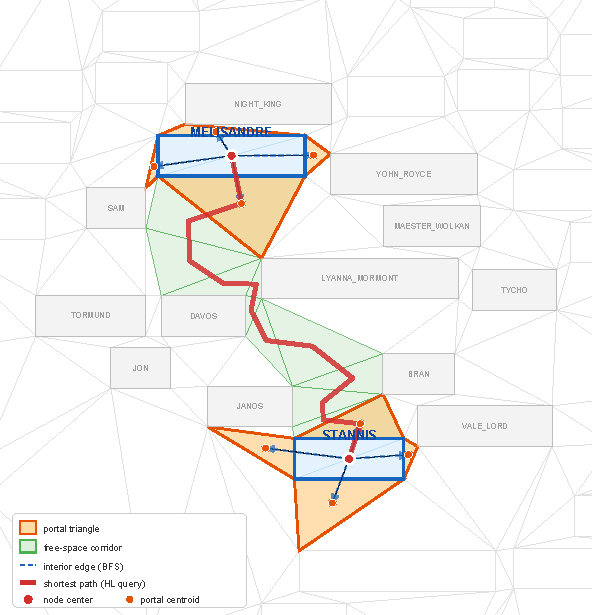
\includegraphics[width=0.75\textwidth]{portal_graph_melisandre_stannis.pdf}
  \caption{The portal graph for the MELISANDRE--STANNIS edge on the Game of Thrones social network. Orange triangles are portals---free-space CDT triangles adjacent to the obstacle boundary. Blue dashed arrows show interior edges from node centers to portal centroids. Green-shaded triangles form the free-space corridor found by the batched Dijkstra search. The thick red polyline shows the shortest path $c_{\text{MEL}} \to p_i \to \cdots \to p_j \to c_{\text{STAN}}$. Nearby node obstacles are shown in gray.}
  \label{fig:portal-graph}
\end{figure}


%% ═══════════════════════════════════════════════════════════════════
\section{WebGL Rendering}
\label{sec:webgl}

The WebGL renderer uses deck.gl~\cite{deckgl}, a GPU-accelerated framework for large-scale data visualization. The renderer sets up an \texttt{OrthographicView} (no perspective distortion) and a \texttt{TileLayer} that dynamically loads tile data based on the current viewport.

\paragraph{Tile resolution mapping.}
The root tile size is rounded up to the nearest power of two. A \emph{start zoom} level is computed so that the root tile maps to the standard 512-pixel tile size of deck.gl. The \texttt{TileLayer}'s \texttt{getTileData} callback translates deck.gl tile coordinates $(x, y, z)$ to \msagljs{} tile map coordinates, fetching the precomputed tile data.

\paragraph{Rendering layers.}
Each tile is rendered as a composite deck.gl layer containing:
\begin{itemize}
\item A \textbf{GeometryLayer} for node shapes (rectangles, ovals, diamonds).
\item A \textbf{TextLayer} for node labels.
\item A custom \textbf{CurveLayer} for edge paths, supporting cubic B\'ezier curves, arcs, and line segments via GPU-side interpolation. Curve tessellation resolution scales with zoom: at zoom level~$z$, the resolution is $2^{z-2}$ segments per curve span.
\item An \textbf{IconLayer} for edge arrowheads.
\item A \textbf{TextLayer} for edge labels.
\end{itemize}

\paragraph{Style-based filtering.}
A declarative style specification allows per-layer control of visibility ranges (\texttt{minZoom}, \texttt{maxZoom}), colors, opacity, sizes, and filters. Styles can reference the node's PageRank to, e.g., show labels only for important nodes at medium zoom levels.

\paragraph{Interaction.}
The renderer supports pan, zoom, hover highlighting, and click selection. Hovering an edge highlights it and its incident nodes. The \texttt{zoomTo} API animates the viewport to a target rectangle with smooth transitions.

%% ═══════════════════════════════════════════════════════════════════
\section{Experimental Results}
\label{sec:experiments}

We evaluate the corridor routing method on benchmark graphs from the Game of Thrones social network~\cite{beveridge2018game}, the GD~2011 contest~\cite{composers}, the Graphviz test suite~\cite{b103,b100}, and the Gnutella P2P network~\cite{gnutella}. All experiments run in Node.js on a laptop with an Apple M1 processor. Layout uses Pivot MDS; timings include CDT construction, routing, and curve smoothing.

Table~\ref{tab:perf} reports the performance of the Dijkstra-tree corridor router (Section~\ref{sec:dijkstra}). For each graph, we report the number of CDT triangles, free-space triangles, the total number of portal triangles across all nodes, and the total routing time.

\begin{table}[t]
  \centering
  \scriptsize
  \setlength{\tabcolsep}{3pt}
  \begin{tabular}{@{}lrrrrrr@{}}
    \hline
    Graph & Nodes & Edges & CDT\,$\triangle$ & Free\,$\triangle$ & Portals & Dijkstra\,(ms) \\
    \hline
    GoT~\cite{beveridge2018game} & 407 & 2\,639 & 3\,258 & 2\,444 & 1\,628 & 277 \\
    b103~\cite{b103} & 944 & 2\,438 & 7\,554 & 5\,666 & 3\,776 & 754 \\
    b100~\cite{b100} & 1\,463 & 5\,806 & 11\,706 & 8\,780 & 5\,852 & 2\,120 \\
    composers~\cite{composers} & 3\,405 & 13\,832 & 27\,242 & 20\,432 & 13\,620 & 9\,335 \\
    Gnutella04~\cite{gnutella} & 10\,876 & 39\,994 & 87\,010 & 65\,258 & 43\,504 & 93\,760 \\
    \hline
  \end{tabular}
  \caption{Corridor routing benchmarks. Dijkstra: per-source Dijkstra trees on the CDT dual.}
  \label{tab:perf}
\end{table}

The Dijkstra-tree approach scales to graphs with tens of thousands of edges. Routing the full Gnutella04 graph (10\,876 nodes, 39\,994 edges) on an Apple M1 laptop takes about 94\,s, which is amortized in interactive use because tile pyramids cache the routes computed at the finest level and rerun only the per-level A* described in Section~\ref{sec:tiling} on coarser zooms.

%% ═══════════════════════════════════════════════════════════════════
\section{Conclusion}
\label{sec:conclusion}

We presented \msagljs{}, an open-source TypeScript library for graph layout, edge routing, and visualization in web browsers. The corridor routing method routes edges directly on the CDT dual graph using a portal graph abstraction and the funnel algorithm. The tiling scheme enables map-like exploration of large graphs with level-of-detail filtering and edge simplification. The WebGL renderer, built on deck.gl, provides smooth pan-and-zoom interaction.

\msagljs{} is available at \url{https://github.com/microsoft/msagljs} under the MIT license.

\bibliography{main}

\end{document}
